%%%%%%%%%%%%%%%%%%%%%%%%%%%%%%%%%%%%%%%%%%%%%%
\logvartrue
\chapter{New tools for new data: comparative genomics software}
%%%%%%%%%%%%%%%%%%%%%%%%%%%%%%%%%%%%%%%%%%%%%%

The quick development of the next generation sequencing technologies have posed serious challenges for the analysis of the high quantity of data produced: new softwares being able to catch up with the technological progress are therefore needed, not only for raw analysis purposes, but also for the constant need to draw a comprehensive picture of the cellular processes and their genetic and molecular components. The first part of this thesis will therefore be focused on the development of two tools dedicated to the analysis of highthroughput technologies data: the objective of these softwares are an easier analysis on these complex new data and, most importantly, the combination of different data sources in the construction of a detailed view on cell biology. A particular focus has been put towards the so-called \textit{usability}, meaning that the developed software should be easy to use and well documented, features that are usually not implemented in most of the now available bioinformatic programs \cite{corpas2012not}. The problems addressed by the two softwares described in this section are the ability to gain structural insights from draft genomes and the ability to provide genetic explanations to phenotypic differences; examples of the utilization of these softwares can be found in Appendix \ref{sec:appendix1}.

\section{The challenges of the \textit{omics} technologies}
\subsection{Improvement of draft genomes using reference genomes}
\begin{figure}[!tb]
	\center
    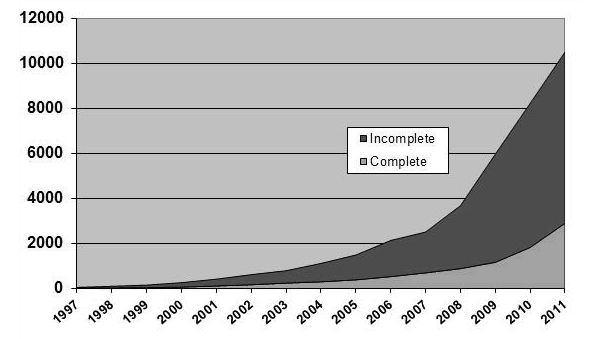
\includegraphics[width=0.7\textwidth]{figures/2/thesis_20}
	\caption{\label{fig:golddraft}\textbf{Sequencing status of the genomic projects}\\
			Number of genomic projects in draft or completed form registered in the GOLD database, October 2011 (from \cite{gold})}
\end{figure}

The recent increase in the number of bacterial genomes available has not seen an equal increase in the number of \textit{finished} genomes, meaning that often the sequences will remain in the so-called \textit{draft} form, as a series of contigs; in fact, most of the recent new genomic projects are submitted in their draft form and are most probably not going to be closed at all \ref{fig:golddraft}. A genome in draft form it's still usefull for genomic and comparative genomics studies, since most of the ORFs can still be predicted with sufficient accuracy (and some gene annotators softwares can handle the ORFs prediction on draft genomes \cite{hyatt2010prodigal}); what is missing it's the possibility to perform structural genomics analysis or to precisely determine the number of replicons and their size. This considerations lead to the need for a new software that would have speeded up the genome finishing phase, with also the ability to gain structural insights from closely related genomes for all those bacterial genomes that would have remained permanently in the draft form.

\subsection{The missing link between genomics and phenomics}
Another key objective in modern biology is the ability to understand the genetic and molecular basis of the phenotypic variability observed in the bacterial kingdom, even inside the same taxonomical unit, such as genera or species. Old molecular techniques allowed the analysis only on small subsets of genotypes and phenotypes for each iteration; however, the advances in the genomic science allow biologists to define the entire genotype of a defined species, while new recent developments in the young field of highthroughput phenomics now allow to obtain a detailed phenotypic picture with relatively limited effort (see for instance the Phenotype Microarray technology \cite{biologPM}). Even though the ability to obtain complete genotypes and sufficiently detailed phenotypes is now easier, to date no tools are available for a comprehensive analysis on the combination of both datasets; indeed some frameworks are already able to provide a skeleton for such studies, like the KEGG metabolic networks, in which both the enzymes mapped in a genome and a series of compunds can be used and linked together \cite{ogata1999kegg}, and may be used to provide clues on the genetic explanations of the phenotypic variability.

\newpage
\section{CONTIGuator: a bacterial genome finishing tool for structural insights on draft genomes}
As discussed in the introduction, one of the main drawbacks of the recent sequencing technologies revolution is the fact that the finishing step is still time consuming and poorly automated, having to rely on an often huge number of PCR reactions to close the remaining gaps between the obtained contigs. Having a closed genome is important to draw a precise functional picture of the strain, because all the ORFs (as well as other functional elements) can be predicted; most importantly, a closed genome is needed for structural genomics analysis, as well for comparative structural genomics. However, since the rate (and cost) of genome finishing it\'s not expected to catch up with the rate of genome sequencing, there is the strong need for computational approaches that allow both an easier way to design the PCR reactions for gap closure and the possibility to predict the functional features of the genome using only the draft sequence. An additional degree of complexity is given by the fact that many bacterial genomes are constituted by more than one replicon, a feature that most of the available programs do not address, leading to less accurate maps for this particular kind of genomes. 
The CONTIGuator software was designed and developed to address these issues: the contigs that constitute the draft genome are mapped to closely related reference genomes, in order to infer their relative orientation, as well to highlight putative structural features. The output of the program comprise a series of structural maps (viewable through the sanger Artemis Comparison Tool \cite{carver2005act}), and a set of primers, which could help in reducing the number of PCR reactions that are needed to close the gaps between each contig.
The software was compared to existing solution, showing that in many cases there was a substantial gain in the the number of bases mapped to the target genome, as well as an higher number of putatively closed gaps.
\newpage
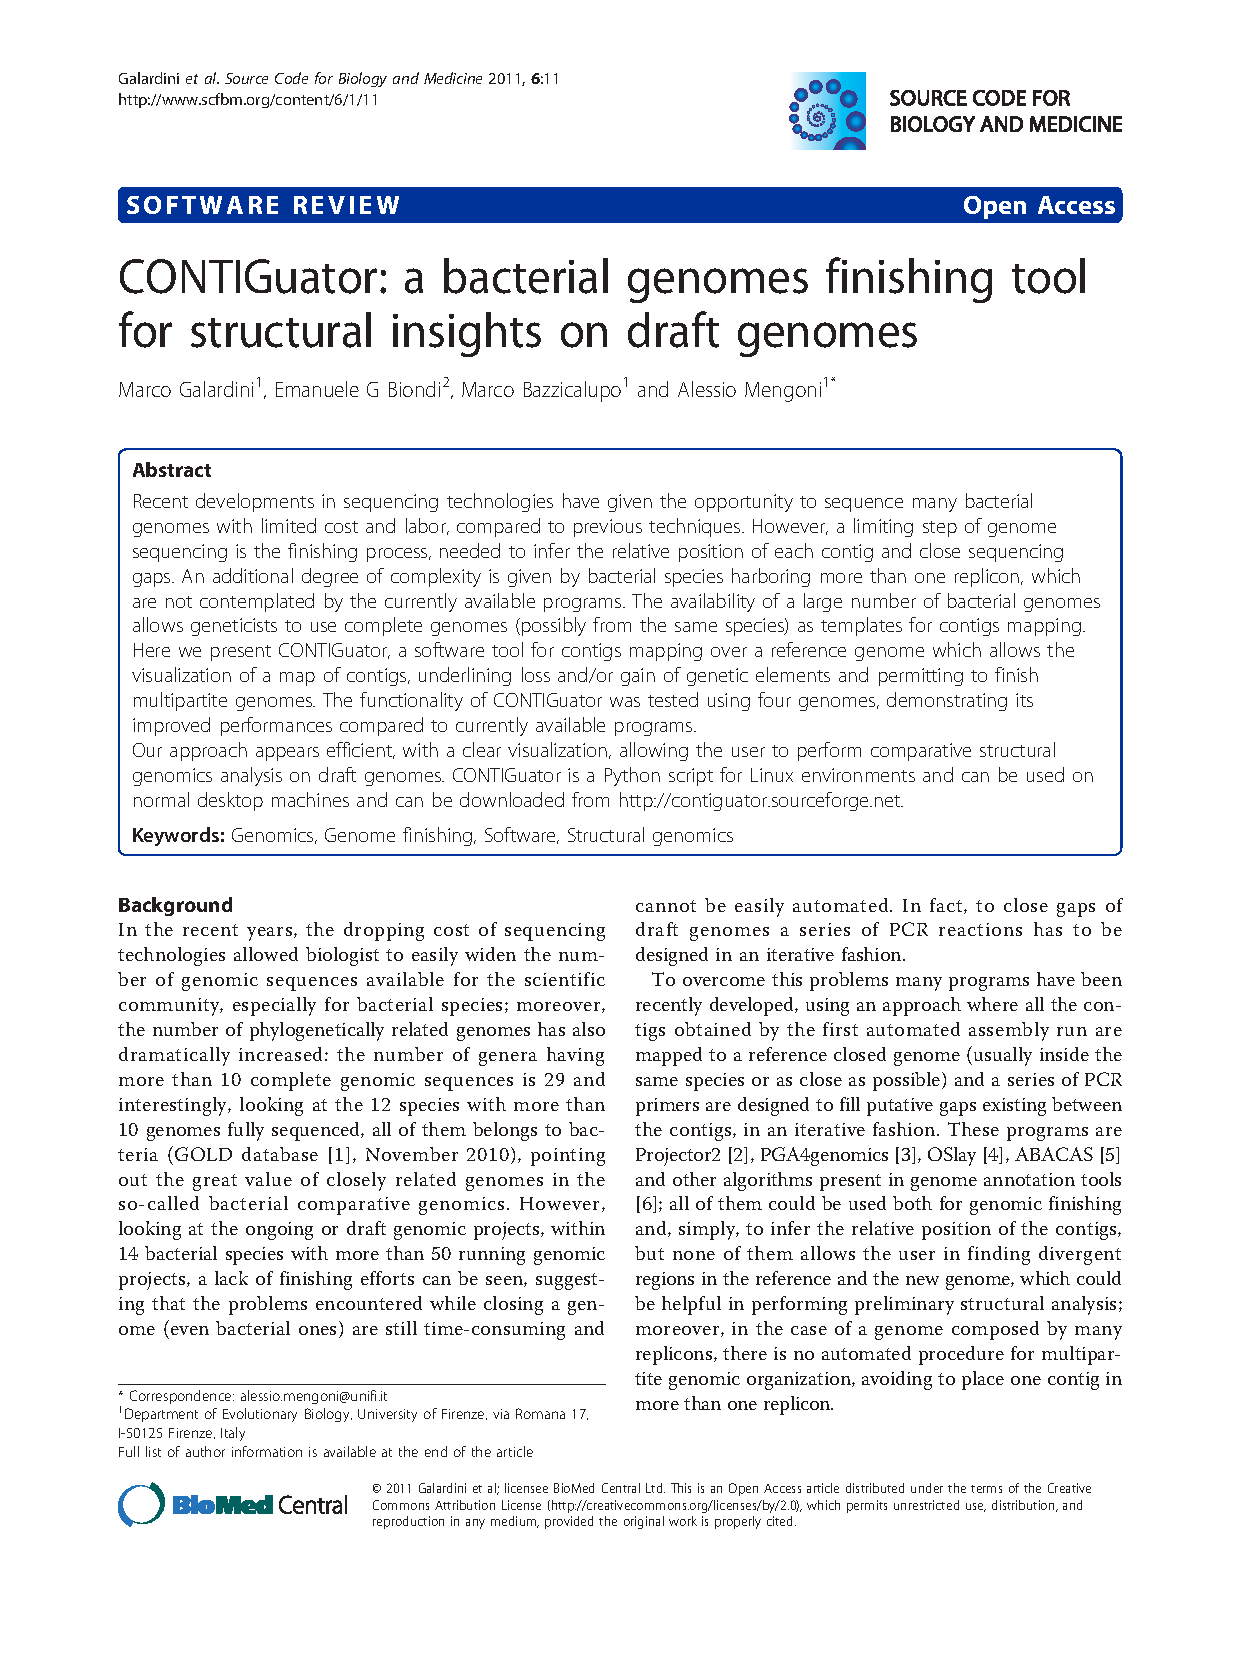
\includepdf[pages=-,offset=10mm 0, scale=0.9]{articles/Galardini2011b.pdf}

\newpage
\subsection{Further developments: version 2 and the CONTIGuator web server}
\begin{figure}[!b]
	\center
    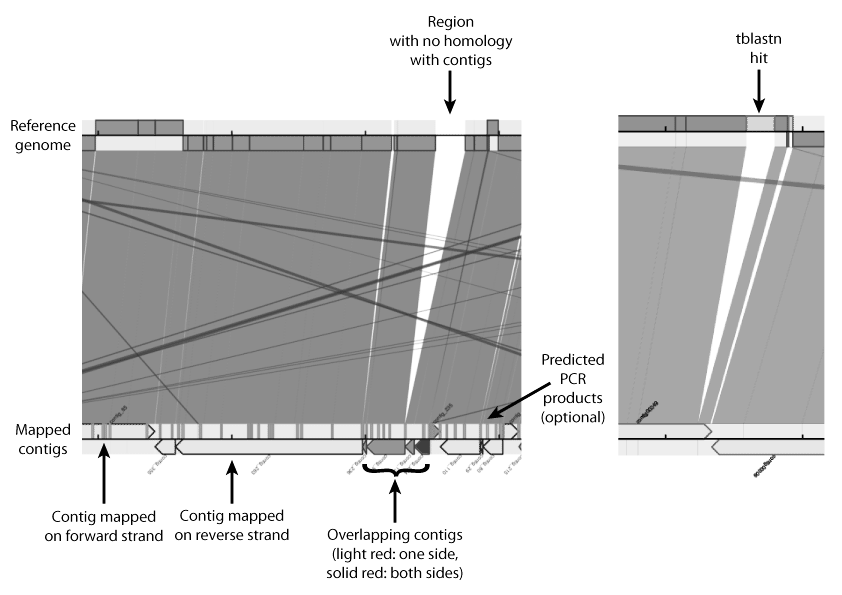
\includegraphics[width=0.9\textwidth]{figures/2/thesis_25}
	\caption{\label{fig:contiguator2}\textbf{CONTIGuator 2 contig maps legend}\\
			from \cite{contiguator}}
\end{figure}

Even though the first version of CONTIGuator was able to provide the needed informations for a faster finishing phase and for a first structural insight, good programming pratices dictate a continuos curation on software features, performances and a prompt bug fixing, together with a continuos enhanchment of the usability and results visualization. The constant help of the scientific community has lead to the second version of CONTIGuator, in which many bugs caused by genomes with peculiar features (like the presence of contigs spanning on the starting point of the reference genome sequence) have been fixed, as well as compatibility with older and newer versions of all the software needed by the program (such as primer3 \cite{rozen2000primer3}, biopython \cite{cock2009biopython} and blast \cite{camacho2009blast+}). The main improvements however, are in the output formats and in the usability features: many new files are produced by the program in order to help a faster analysis on those contigs that have been mapped by the program and those that are not mapped; also the contig maps, that are necessary to gain the structural insights have been improved, with a faster and automated launch of the ACT \cite{carver2005act} program and the generation of static maps in pdf format, thanks to the GenomeDiagram package inside biopython \cite{cock2009biopython}\cite{pritchard2006genomediagram}, which are best suited for exchange and publications (Figure \ref{fig:contiguator2}).

\begin{figure}[!tb]
	\center
    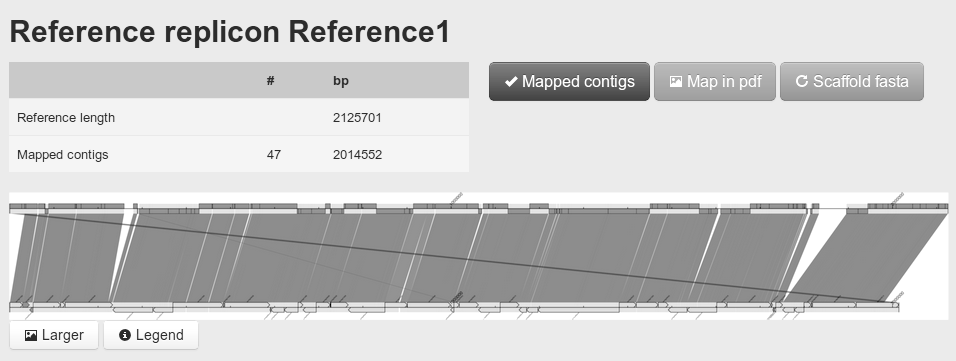
\includegraphics[width=0.9\textwidth]{figures/2/thesis_26}
	\caption{\label{fig:contiguatorweb}\textbf{The CONTIGuator web interface results page}\\
			from \cite{contiguator2}}
\end{figure}

A further step forward in terms of usability has been the development of a web interface to the program, which allows users that are not experts in the field of bioinformatics to use the program and to analyze the results: the software features are the same as the regular command line version, but from the user perspective, there is no need to install any program or to learn any bioinformatic skills (Figure \ref{fig:contiguatorweb}). In fact the number of users that have used the program since September 2012 to December 2012 are more than one hundred. 

\newpage
\section{DuctApe: a tool for analysis and correlation of genomic and high throughput phenotype data}
\label{sec:ductape}
Understanding the functionality of genomes is one of the most important and challenging tasks of today's biology. In particular the linkage between genomes and corresponding phenotypes (i.e. metabolic abilities) is of particular interest in the reconstruction and biotechnological modification of metabolic pathways and also in the study of their evolution. In the last years, the Omnilog\texttrademark Phenotype Microarray (PM) technology has been used to address many specific issues related to the metabolic functionality of microorganisms. However a software which could directly link PM data with the genome(s) of interest, then extracting the information on gene-phenotype correlation is still missing. Fot this purpose DuctApe was developed, a software tool that allows to analyse genome sequences and PM data, finding and visualize any metabolic difference among PM experiments and to correlate them with KEGG pathways and gene presence/absence patterns.

Source code and tutorial are freely available on \href{http://combogenomics.github.com/DuctApe/}{GitHub} (@combogenomics). DuctApe is written in Python and can be installed in UNIX environments\footnote{Authors: \textbf{Marco Galardini}, Alessio Mengoni, Emanuele G. Biondi, Alessandro Florio, Marco Bazzicalupo, Stefano Mocali}.

\subsection{Introduction}
In the recent years the continue development and success of new sequencing instruments, (so-called ”next generation” or ”massively parallel"), have exponentially increased the high-throughput DNA sequencing which is becoming available and affordable even for small labs, which are potentially able to sequence hundreds of bacterial strains per year \cite{metzker2009sequencing}. Actually the reduced time and costs of genomic analysis have already allowed the achievement of over 2100 prokaryotic complete sequences (on October 2012). Although a number of other “omics” techniques have determined a terrific contribution to address fundamental biological questions in microbiology (i.e. transcriptomics, proteomics, metabolomics, metagenomics, etc.) \cite{zhang2010integrating}, the cell phenotype represent the final expression of the genomic information and the result of all the components described by the previously addressed “omics” techniques. Furthermore, most of the genes from genomic sequencing efforts have no ascribed function, and even genes with ascribed functions are based primarily on DNA sequence homology, with little or no direct experimental data \cite{mardis2008impact}. In order to assess a rapid functional and phenotypic profiling under different conditions, a high-throughput approach was developed by BIOLOG Inc. (Heyward, CA): the Phenotype Microarray (PM) technology. PM technology, based on the OmniLog\texttrademark platform, is a system designed for metabolic and antibiotic resistance assays of both bacterial and eukaryotic strains in 96-well PM plates comprising a total of 2400 physiological challenges under temperature-controlled conditions. In each well the physiological reaction can be monitored using cell respiration as a reporter system. Indeed if the cell can catabolize the substrate there will be a flow of electrons from the carbon source to NADH, which determines the reduction of a tetrazolium violet dye and the consequent production of a purple colour (formazan) \cite{bochner2001phenotype}. The colour change is then recorded by an automatic camera every 15 minutes, providing a huge amount of data over the course of several days. These data are directly stored in the computer and can be analyzed by means of OminoLog\texttrademark PM software \cite{biolog2009}. However, managing the data produced in these experiments is not immediate and practical. Some software, which could enhance the tools supplied with the OmniLog\texttrademark instrument have been proposed, such as PhD database \cite{li2005phd}, the RetroSpect\texttrademark software \cite{biolog2008} and PheMaDB \cite{wenling12phemadb}. However such applications are mainly customized databases which have been developed for the management and the storage of phenotypic data obtained from the OminoLog\texttrademark PM software, which displays the PM measurements as 96-wells plate layout and provides few single kinetic parameter values from each curve, without considering the entire curve shapes and kinetics. In fact, as recently highlighted by Vaas and co-workers (2012), the PM respiration kinetics contain additional valuable biological information that go significantly beyond the mere presence/absence measurements and which need to be better exploited. In their work the authors proposed a R-based software solution (package \textit{opmdata}) for exploiting multiple respiration curves from PM data and providing also a detailed statistical estimation of the results. Although the visualization of the PM raw data was significantly improved as compared to the native Omnilog\texttrademark PM software, unfortunately any useful tool for linking the results to putative metabolic pathways is  provided. Nevertheless a tool for comparing and linking genomic and phenomic data is also unavailable. The opmdata package provides four parameters for each growth curve, which is useful for a deeper analysis on single curves; however, such a multidimensional approach doesn't allow a direct way of comparison of entire datasets, or the inclusion of the phenotypic information inside the metabolic network. To better face this challenge and fill this gap we have designed an easy-to-use software system called DuctApe, which links together both the genomic and the phenomic data and suggests genetic explanations of metabolic phenotypes. The software uses the KEGG database as a source of information for metabolic pathways, divided in reactions (that are the proteins in each genome) and compounds; this is where DuctApe comes to help, mapping the genome content and the compounds into the same metabolic maps. It also provides various network statistics to help predict which parts of the metabolic network may be more related to the utilization of a specific compound. Furthermore, several kinds of experimental setups can be analyzed: 

\begin{itemize}
\item single strain experiment,
\item mutational experiments with one reference strain and one or more mutants,
\item pangenomic experiments with more than one organism simultaneously.
\end{itemize}

Several works have been published to assess the link between genomic and PM data \cite{biondi2009metabolic}\cite{viti2009involvement}\cite{peleg2012success} or attempted to improve genome annotation \cite{reed2006towards}, but the managing of data produced in these experiments did not cover all the potential information within the dataset. Here, we tested DuctApe on two PM datasets: the first one from four strains of the symbiotic nitrogen-fixing model bacterium \textit{Sinorhizobium meliloti}, determined on PM 1,2,3,4,5,9 and 10 (\cite{biondi2009metabolic}; the second one comprised the same four strains but their phenotype was determined by using the entire OmniLog\texttrademark system plate set and compared to their previously sequenced genomes \cite{galardini2011exploring}.

\subsection{System and methods}
The tool has been developed as a \textit{“suite”}, which is constituted by three individual modules: 1) DuctGenome (\textit{dgenome}): for genomic data analysis; 2) DuctPhenome (\textit{dphenome}): for PM data analysis; 3) DuctApe (\textit{dape}): for genomics and phenomics linking; the third module is also used to manage to setup the experiment and handle the KEGG data.
 
\subsubsection{DuctGenome (dgenome)}
The first module is used to handle the genomic data from the strains of the experiment, and to return the metabolism reconstruction according to the KEGG database, as a series of pathway maps in which the proteins encoded in the genome are mapped and putatively assigned to a metabolic task. The user can directly provide the list of KEGG identifiers (i.e. the KEGG orthology IDs given by the KAAS automatic annotation server \cite{moriya2007kaas}) or a local KEGG database to which the proteins of each organism will be queried through a Blast-BBH, using the Blast+ software \cite{camacho2009blast+}. Once that a list of KEGG identifiers is available, the metabolic network is reconstructed using the KEGG API (Application Programming Interface). The metabolic map reconstruction will be used by the dape module. If a pangenomic experiment is set, the information on the conserved, accessory and unique metabolisms can be extracted through the detection of all the orthologs (the so-called pangenome); the user can provide the orthologs classification as provided by an external algorithm, like InParanoid \cite{ostlund2010inparanoid} or use the internal parallel Blast-BBH approach \cite{popa2011directed}. The protein sequences are handled by the BioPython package \cite{cock2009biopython}.

\subsubsection{DuctGenome (dphenome)}
\begin{sidewaysfigure}
	\center
    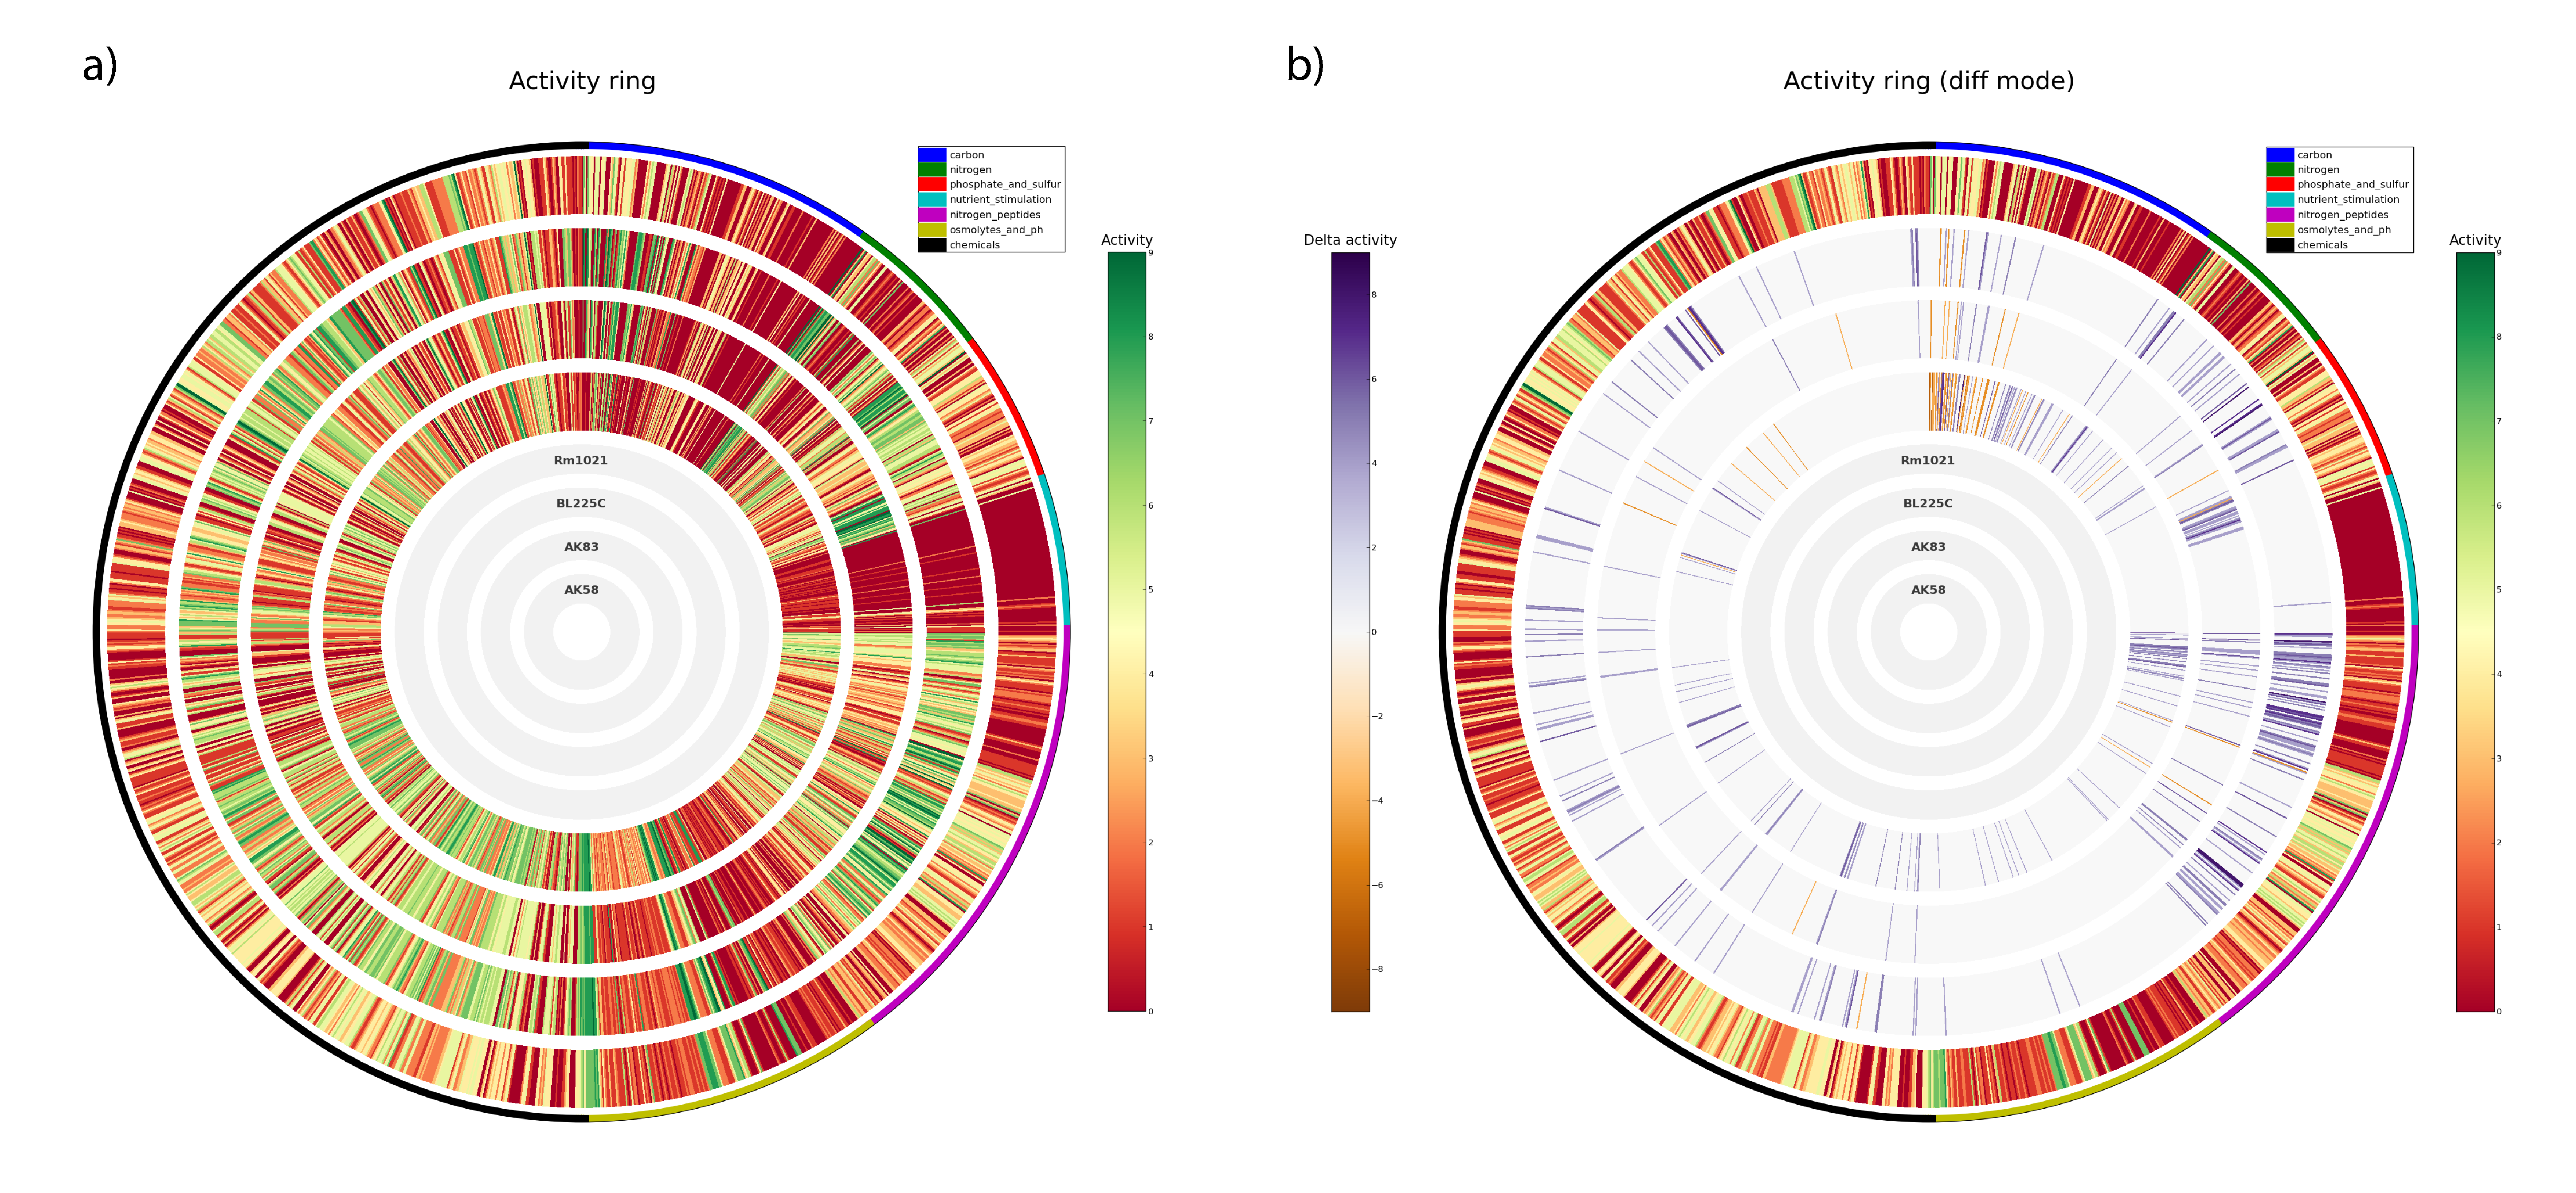
\includegraphics[width=1\textwidth]{figures/2/thesis_21a}
	\caption{\label{fig:drings}\textbf{Activity rings}\\
			Activity rings from \textit{S. meliloti} Phenotype Microarray data; grey inner circles indicate the strains order\\
			a) The Activity Index (AV) calculated for each strain and well is reported as a color going from red (0 AV) to green (9 AV)\\
			b) Diff mode: the difference with the AV value of strain Rm1021 is reported when equal or higher of 3 AV, grey otherwise; purple colors indicate an higher activity with respect to Rm1021, orange colors a lower activity}
\end{sidewaysfigure}

This second module allows the user to provide and manage any kind of phenomic data that can be linked to the KEGG compound database: a special focus is on PM data, for which a series of additional analysis tools are present, from raw data parsing to automatic activity calling and results plotting. In order to avoid any unreasonable or uninterpretable biological result displayed by using different parameters in certain situations and estimated to be up to 36\% of data \cite{vaas2012visualization}, for each well of the multiwell plate of the OmniLog\texttrademark system plate set, the \textit{Activity Index} (AV) is here proposed as a concise parameter based on the length of the lag phase, the slope of the curve, the average height, the maximum cell respiration and the area under the curve. Such index could provide both qualitative (presence/absence) and qualitative (model fitting data) information. First of all it is necessary to insert the output PM data from the Omnilog software: several files in csv format with raw data (in-cluded replicas) can be used. The program can then follow the steps below:

\begin{enumerate}
\item Parsing
\item Control signal subtraction
\item Signal refinement (smoothing)
\item Parameters extraction 
\item Activity Index calculation
\item Replica management
\item Growth curves plots 
\end{enumerate}

The data is parsed by the program and stored inside the project file; the user can then decide if the control signal has to be subtracted, or if a \textit{blank} plate (with no inoculants) should be used for this purpose, since some concerns regarding the control signal subtraction have been recently issued \cite{vaas2012visualization}. The PM curve parameters are extracted through the fit of one of three sig-moid functions (Logistic, Gompertz, Richards), reformulated to facilitate the parameters extraction \cite{zwietering1990modeling}; in order to avoid incorrect fittings or even failures, the growth curve signal is smoothed through the application of the Blackman window approach, as implemented in the SciPy package \cite{jones2001scipy}, which is also used to perform the actual fit. If all the three functions cannot be fitted to the PM curve, up to two more rounds of signal smoothing are applied; if the curve fit cannot be applied even after three rounds of smoothing, that particular well is classified as not active and the plateau, slope and lag parameters are set to zero.
The so-called Activity Index (AV) is a value between 0 and 9, which indicates those wells that exhibit low or none metabolic activity (0) and those with high metabolic activity (9) inside that par-ticular experiment: the AV parameter is calculated through a k-means clusterization (with k=10) on five growth curve parameters (max, area, height, lag, slope); the low activity growth curves will be assigned to the clusters with low AV, while wells exhibiting higher metabolic activity will be assigned to clusters with higher AV. The MeanShift clustering algorithm is also applied, in order to verify that there is a real clusterization of the growth curves in distinct clusters, as this algorithm has no fixed amount of clusters. The clusterization is performed with the scikits.learn package \cite{pedregosa2011scikit}. Since in most of the cases, many copies of each plates are used, there may be also the need to highlight those growth curves whose behavior is significantly different from the average: the program can search for those replica that are distant from the average AV (for that particular well and strain) more than an user-defined AV delta and flag them as \textit{purged}, meaning that they are not considered in the other analysis. The program has four replica purging policies, to help the user decide which PM curves have to be maintained. The last operation on the Phenotype Microarray data is the generation of PM curves plots with the matplotlib package \cite{hunter2007matplotlib}, which, compared to those generated by the machine vendor software, allow the comparison of more than two strains at the same time, with plate-wise plots, single wells plots and plate-wise AV heatmaps. Moreover it is also possible to display the entire metabolic profile of one or more strains in an interactive ring-mode view, called the “Activity ring”. Such graphical representation could report either the total Activity Index values (Figure \ref{fig:drings}a) or the metabolic differences between any selected sample versus the other strains by providing a "diff mode" Activity ring which displays the information by metabolic category of tested strain by using different colour intensity (Figure \ref{fig:drings}b). The values of the differences are represented by colour intensity (blue and orange parts indicate higher and lower values, respectively). Details of the Activity Index values are reported in a separate file which is directly accessible for the user. Different colors on the external line of the rings indicate different PM compounds categories. These visualizations allow an easier detection of the metabolic categories which are more variable in the tested strains. 

\subsubsection{DuctApe (dape)} 
The data gathered in the first two modules can be analyzed together in the third module of the DuctApe suite, which is designed to construct the metabolic network using the KEGG database information about reactions (which are the proteins mapped by the dgenome module) and compounds (which are the PM compounds, divided in categories); a series of interactive metabolic maps are then prepared, with specific color codes depending on the type of the experiment; the metabolic maps are encoded as a series of web pages that can be explored using a web browser. Using these maps, the user can highlight those pathways in which the gene pres-ence/absence pattern fits with the metabolic activity of the PM compounds. Moreover, thanks to the networkx module \cite{hagberg2008exploring}, several statistics can be computed for the whole reconstructed metabolic network and for each pathway, like the number of mapped reactions, the number and length of connected components (that are in fact distinct and independent metabolic modules) and the average AV for the total metabolic network and each pathway. Such analysis are useful for quick comparisons between various strains, moreover, the whole metabolic network graph is saved in gml format for further analysis on graphs visualization software like Gephi \cite{bastian2009gephi}.

\subsection{Results}
\subsubsection{Evaluation of dgenome on biological data}
\begin{figure}[!tb]
	\center
    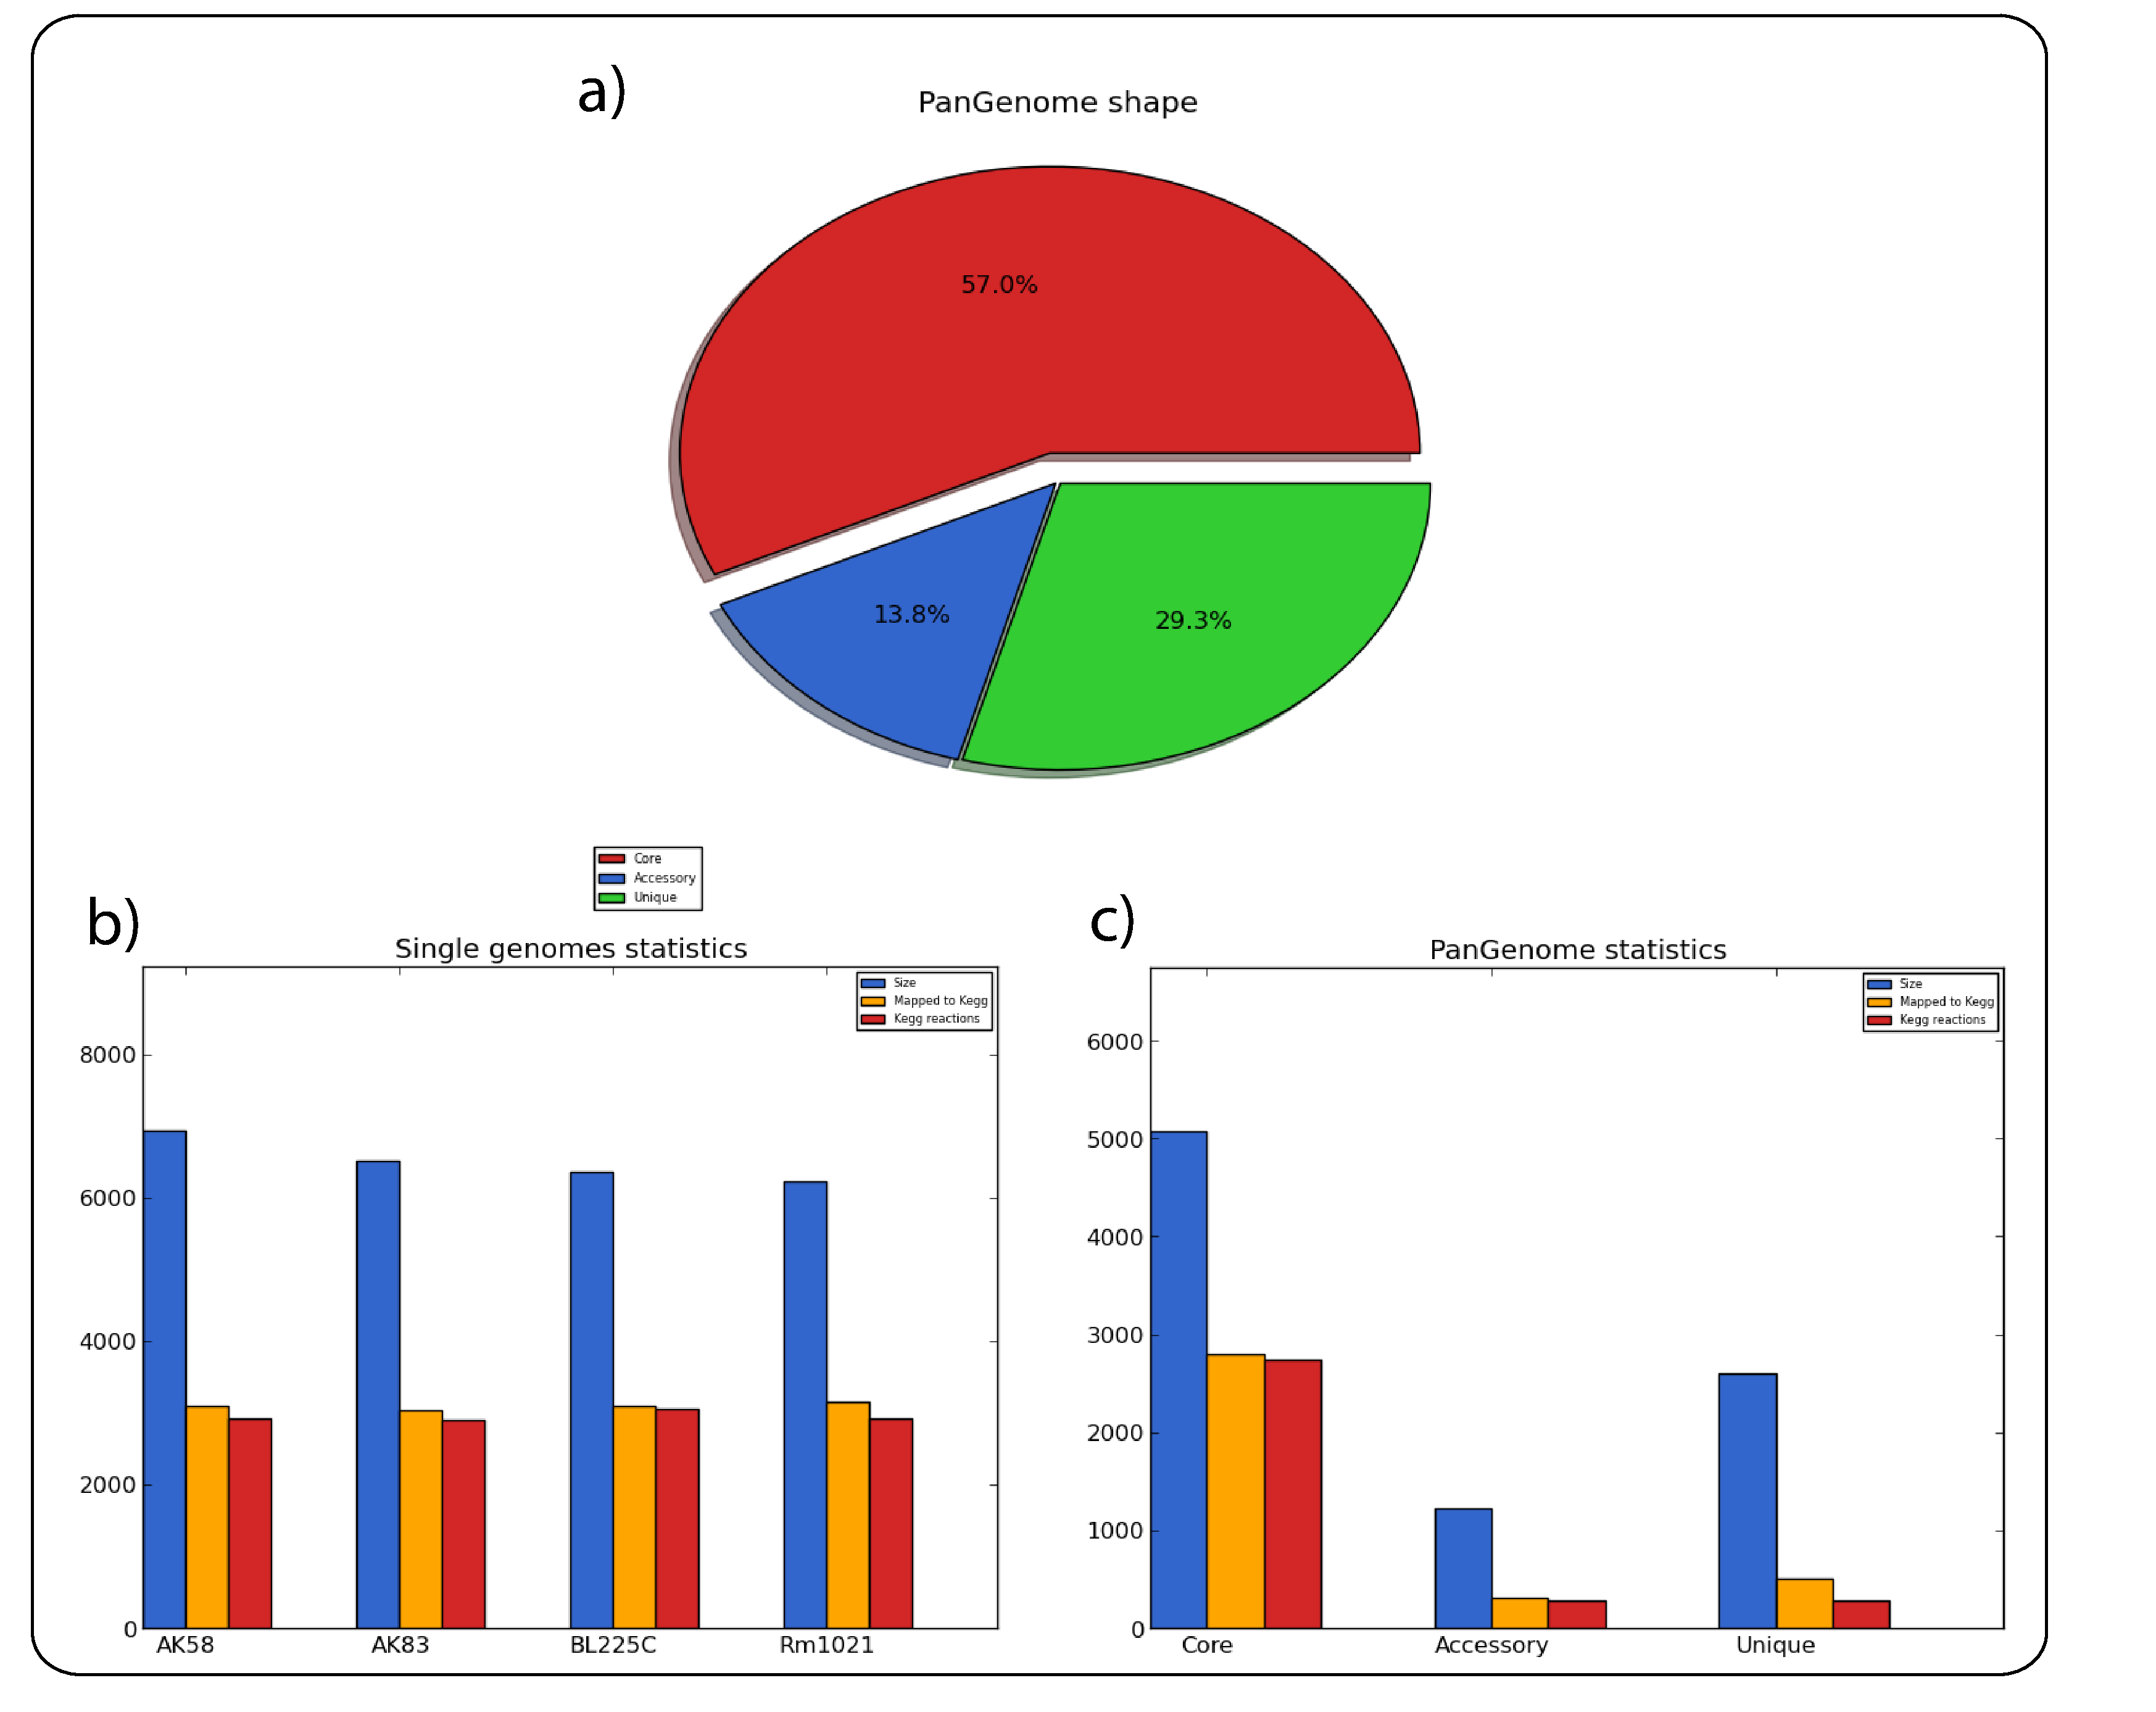
\includegraphics[width=0.9\textwidth]{figures/2/thesis_22}
	\caption{\label{fig:dgenome}\textbf{Pangenome statistics}\\
			a) The partition of the calculated pangenome in terms of core, accessory and unique genes\\
			b) Proteome sizes of the four S. meliloti strains and the fractions of proteins mapped to KEGG and KEGG reactions\\
			c) Pangenome partitions sizes in number of orthologous groups and fraction of orthologs mapped to KEGG and KEGG reactions}
\end{figure}

The four \textit{Sinorhizobium meliloti} strains used for this example study (Rm1021, AK83, AK58 and BL225C) were previously sequenced \cite{galibert2001composite}\cite{galardini2011exploring} and their predicted proteins were mapped to KEGG using the KAAS annotation web server, while the strains pangenome was computed thanks to the dgenome Blast-BBH algorithm; this resulted in a pangenome with 5074 orthologous groups belonging to the core genome, 1227 to the accessory fraction and 2606 unique to a single strain (Figure \ref{fig:dgenome}a). When looking at the number of proteins mapped to KEGG reactions, a similar number of proteins were mapped in each of the four genomes (Figure \ref{fig:dgenome}b), while when looking at the pangenome, the highest fraction of proteins mapped to KEGG come from the core genome, with a limited fraction of reactions mapped in the accessory and unique genome (Figure \ref{fig:dgenome}c).

\subsubsection{Evaluation of dphenome on biological data}
The first aim was to provide a rough evaluation of the Activity Index and its reliability. In order to do that the analysis and the comparison of the first PM dataset obtained from a previous experiment focused on 4 strains of the symbiotic model bacterium \textit{Sinorhizobium meliloti}: Rm1021, AK58, AK83, BL225C \cite{biondi2009metabolic} has been carried out. Such phenotipic dataset was obtained on the four strains by using the OmniLog\texttrademark system with plates PM1, 2, 3, 4, 9 and 10, and the metabolic variability was compared by means of the ratio between the average area and the area under the curve among strains for each condition. PCA and cluster analysis confirmed that the metabolic distance between Rm1021 and the other strains appeared to be quite consistent with the previous work, although it also provided slight differences involving strain AK58. In order to exploit the reasons of such differences, the Omnilog kinetic parameters of slope, maximum height, lag time and area under the curve were also individually analysed. Both PCA and cluster analysis confirmed that all the selected parameters, except the lag time, showed similar results as compared to the Activity Index which could thus be successfully applied as a unique parameter into the dphenome module (Figure \ref{fig:dpca}).

\begin{figure}[!tb]
	\center
    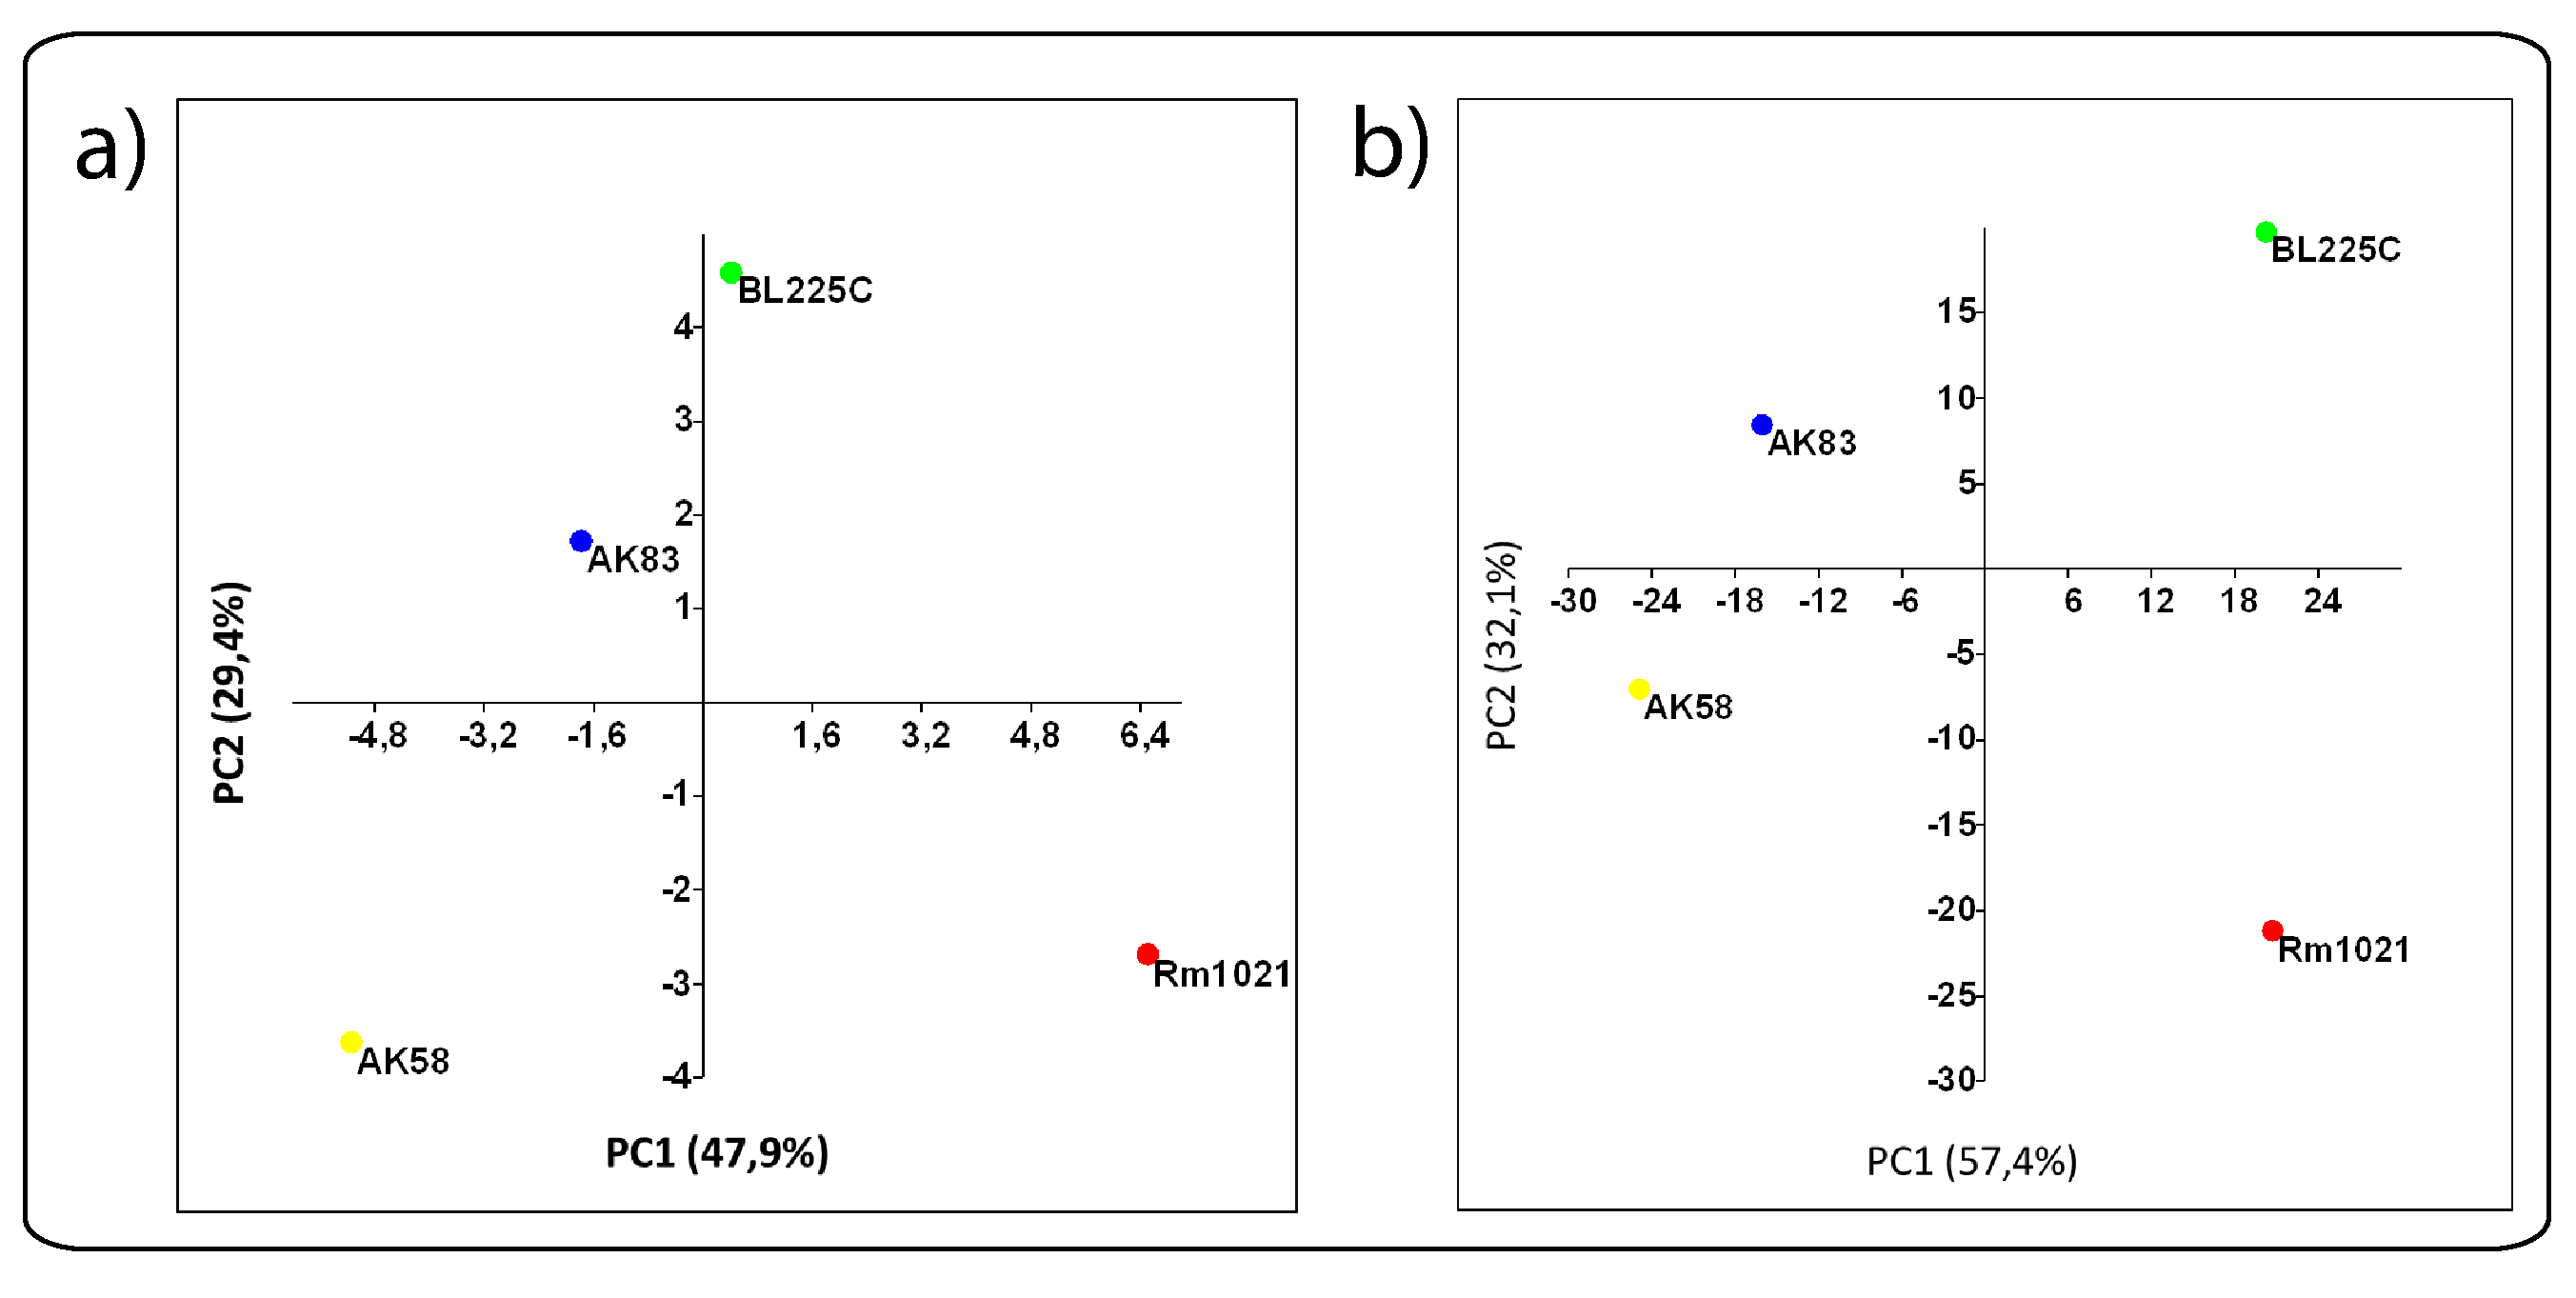
\includegraphics[width=1\textwidth]{figures/2/thesis_23}
	\caption{\label{fig:dpca}\textbf{Evaluation of the Activity Index by comparing the phenotypic diversity of four \textit{S. meliloti} strains}\\
			a) PCA results for PM profiles obtained from the analysis of 517 phenotypic attributes (dataset 2009) expressed as the ratio between the average area and the area under the curve among strains for each condition (see Biondi et al., 2009 for further details)
			b) PCA results for Activity Index values obtained from the PM analysis of the same 517 phenotypic attributes (dataset 2009)}
\end{figure}

\begin{table}[htbp]
  \centering
    \begin{tabular}{rcccc}
    \toprule
          & AK58  & AK83  & BL225C & Rm1021 \\
    \midrule
    More active & 57    & 26    & 70    & 4 \\
    Less active & 40    & 10    & 6     & 88 \\
    Total & 97    & 36    & 76    & 92 \\
    \%    & 5.1   & 1.9   & 4     & 4.8 \\
    \bottomrule
    \end{tabular}%
  \caption{\textbf{Unique metabolic functions of each \textit{S. meliloti} strain}}
  \label{tab:uniquemet}%
\end{table}%2


In order to evaluate the full potential of the dphenome module, the Activity Index was applied to a second phenotypic dataset obtained by a new biological test carried out using the entire OmniLog\texttrademark system PM plate set, and compared to the parameters calculated by the opmdata package \cite{vaas2012visualization}. We also compared the performances of the two approaches, with our parameters extraction taking up to ten minutes to be completed on the whole dataset (20 plates on 4 strains), while the opmdata package can takes up to several hours for the same task. A first qualitative output can be obtained by simply comparing the high/low metabolic activity on each PM well condition between the four strains. As shown in Table \ref{tab:uniquemet}, the 86,7\% of the substrates use was shared between the four strains (difference of Activity Index <3), whereas the 11,1\% of the metabolic repertoire was unique for each of them and could be strongly related to specific genomic traits. The remaining substrates were shared between more than one strain. The highest number of unique “more active” metabolic features was detected in PM plates inoculated with BL225C strain (70), suggesting a higher metabolic potential of this strain as compared to the other three. In fact, the BL225C strain exhibited “less active” phenotypic traits in 6 conditions only. In contrast, the Rm1021 strain seems to be the less metabolically competitive between the four strains, as it showed the lowest number of “more active” metabolisms (4) and the highest number of “less active” metabolisms (88). When looking at the single PM compound categories (Table \ref{tab:ductcateg}), trends highlighted in Table \ref{tab:uniquemet} are confirmed for each category, with strain Rm1021 as the less active in each cate-gory, except for  plates measuring the tolerance to pH and stresses, in which strain AK83 has a lower proportion of active wells com-pared to strain Rm1021.

\begin{sidewaystable}[htbp]
  \centering
  	\begin{tabular*}{\textwidth}{rccccrr}
    \toprule
    \multicolumn{1}{c}{} & \multicolumn{4}{c}{Active wells (\%) *} &       &  \\
    \midrule
    Category & AK58  & AK83  & BL225C & Rm1021 & \multicolumn{1}{c}{Average difference} & \multicolumn{1}{c}{Main differences (\%)** } \\
    Carbon & 14,1  & 20,8  & 22,9  & 14,1  & \multicolumn{1}{c}{1,7} & \multicolumn{1}{c}{22,9} \\
    Nitrogen & 40,6  & 25    & 51    & 19,8  & \multicolumn{1}{c}{1,3} & \multicolumn{1}{c}{5,2} \\
    Phosphate and sulfur & 29,2  & 43,8  & 66,7  & 14,6  & \multicolumn{1}{c}{1,9} & \multicolumn{1}{c}{12,5} \\
    Nutrient stimulation & 1     & 4,2   & 2,1   & 1     & \multicolumn{1}{c}{0,4} & \multicolumn{1}{c}{1} \\
    Nitrogen peptides & 40,6  & 28,5  & 62,8  & 14,6  & \multicolumn{1}{c}{1,7} & \multicolumn{1}{c}{9} \\
    Osmolytes and pH & 25,5  & 17,7  & 22,4  & 19,8  & \multicolumn{1}{c}{0,9} & \multicolumn{1}{c}{1,6} \\
    Chemicals & 41,9  & 39,8  & 47,6  & 17,9  & \multicolumn{1}{c}{1} & \multicolumn{1}{c}{2,8} \\
    \bottomrule
   \end{tabular*} 
  \caption{\textbf{Phenomic data for each Phenotype Microarray compound category}\\
  \textbf{*} compounds for which the AV (activity index) is equal or over 5\\
\textbf{**} compounds for which the average difference between the strains is equal or over 3 AV (activity index)}
  \label{tab:ductcateg}%
\end{sidewaystable}

However, in order to further highlight any metabolic difference between the selected samples it could be also possible to compare the Activity Index of the curves over time. The total metabolic differences of the entire PM dataset was then displayed as an Activity Ring (Figure \ref{fig:drings}a). It could be also visualized as diff mode in order to visually detect any difference in higher/lower metabolic reaction between any selected strain and the other samples. For instance, in Figure \ref{fig:drings}b the relative metabolic differences between Rm1021 and the other strains are shown; a significant increase of blue colour intensity appeared in the “Nitrogen peptides” category, suggesting a lower metabolic activity of Rm1021 as compared to the other \textit{S. meliloti} strains. Thus, the user is free to get further information by accessing a separate file, where the detailed values of Activity Index for each substrate are reported.

\subsubsection{Evaluation of DuctApe on biological data}
\begin{sidewaysfigure}
	\center
    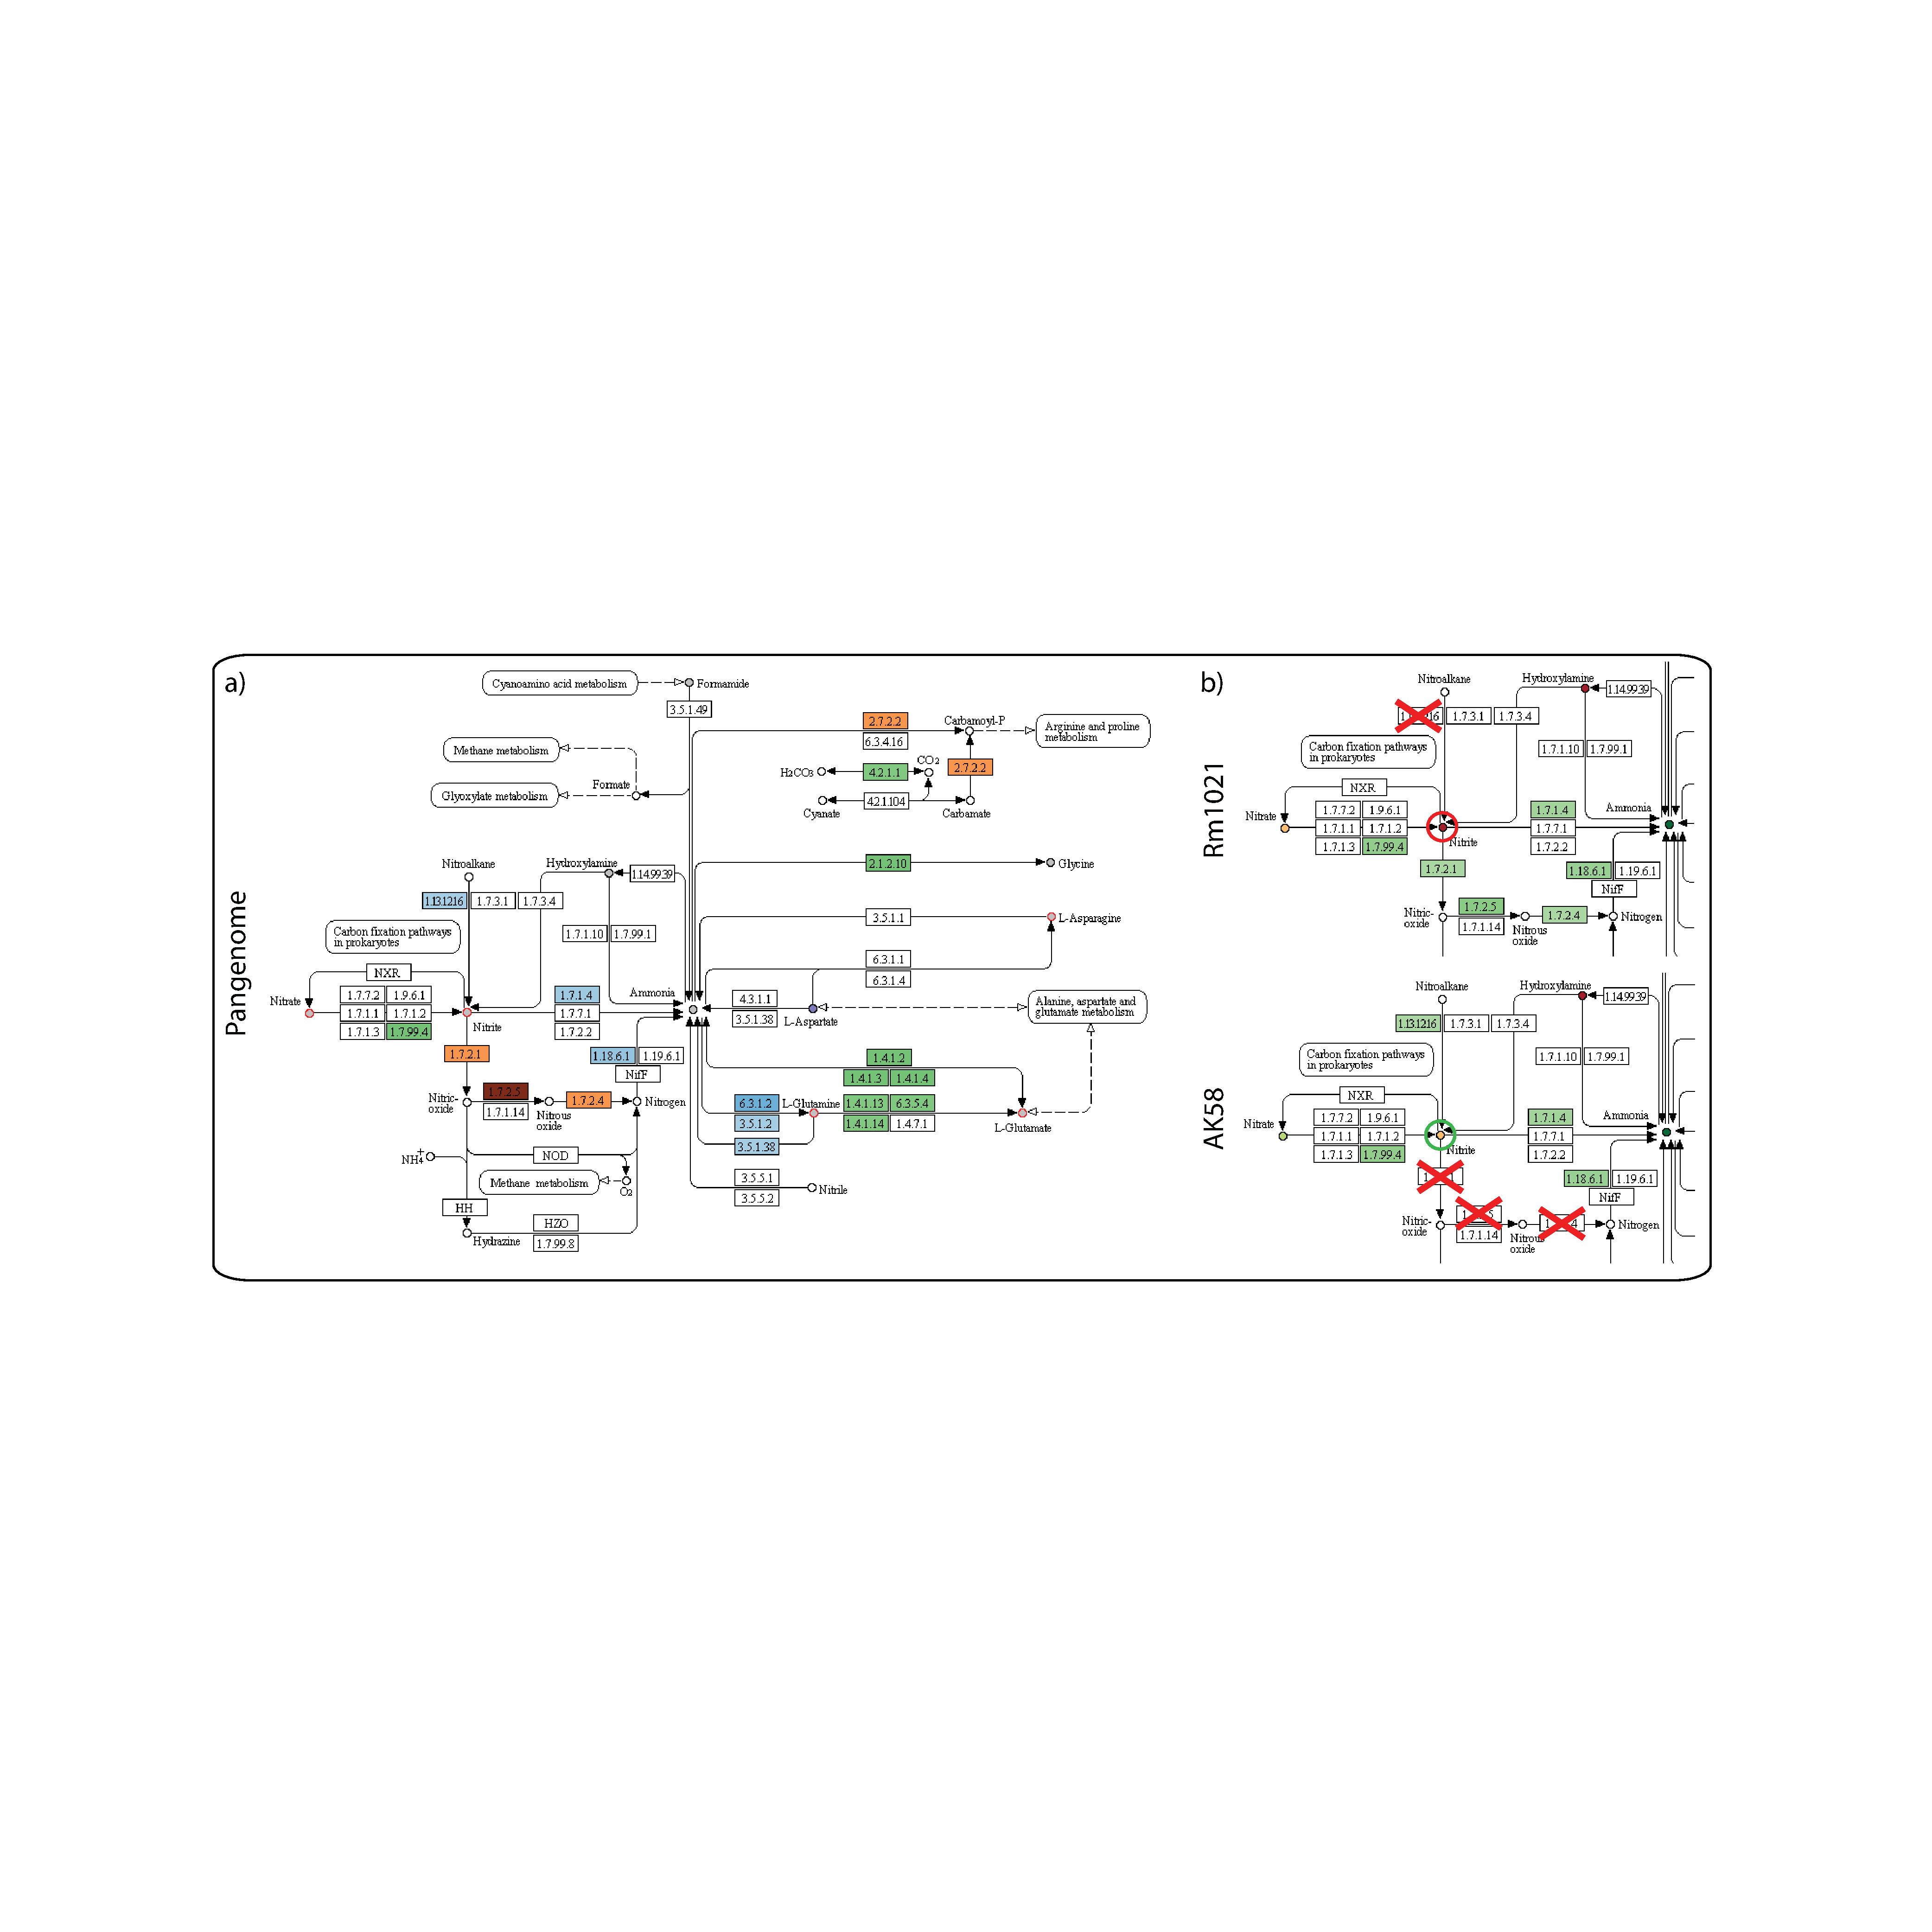
\includegraphics[width=1\textwidth]{figures/2/thesis_24}
	\caption{\label{fig:dkeggmaps}\textbf{Metabolic network analysis on the \textit{S. meliloti} pangenome}\\
			Boxes represent reactions, with color intensity proportional to the copy number, while circles represent compounds\\
			a) Pangenome metabolic map of nitrogen metabolism: core reactions are colored in blue, reactions present both in the core and accessory genome are colored in green, unique reactions are colored in orange; compounds are colored in purple when the mean AV difference in the four strains is equal or higher of 3 AV, grey otherwise. Red circles around grey compounds highlight those compounds for which at least one strain has an AV difference with the other strain equal or higher than 3 AV\\
			b) A section of the same metabolic map in strain Rm1021 and AK58: reactions are colored in green, compounds are colored according to their AV (as in Figure \ref{fig:drings}); differences between the two strains are highlighted with red crosses}
\end{sidewaysfigure}

The schematic representation of the metabolic pathways potentially expressed from each of the four strains was retrieved by selecting the command "dape map". A number of metabolic maps from KEGG database were separately displayed as functional categories for each strain. The different gene-related phenotypes could be analyzed on the basis of the presence of genes and substrates of each map, highlighting them with different colors (as described in Figure \ref{fig:dpca}). However the potentials of DuctApe could be fully expressed in case the user wants to compare the metabolic features of multiple samples. For example in Figure \ref{fig:dkeggmaps}a the pangenomic map for nitrogen metabolism (map n. 00910 of KEGG database) is shown. Although most of the reactions are catalyzed by proteins encoded by genes which were not retrieved from the genomic data (white boxes), some reactions appeared to be controlled by genes of the core genome (blue) or present in both core and dispensable genome (green). Nevertheless, four orange boxes indicated the presence of the following functional genes located on the dispensable genome: nitrite reductase (reaction 1.7.2.1), nitrous-oxide reductase (reaction 1.7.2.4) and carbamate kinase (reaction 2.7.2.2). This means that these functions are not shared between all  strains. In fact those genes were not detected in AK58 and AK83 strains. Similarly, most of the metabolic substrates involved in the nitrogen cycle are not included into the PM microplates set (white circles) but several substrates could be used (or not) by the four strains (colored circles). For instance, all the samples showed active metabolism for some specific substrate (i.e. Ammonia, L-Glutamate, etc.) as well as no active metabolism for some other substrate (i.e. Hydroxylamine, Formamide, etc.) which are indicated with a grey circle on the map. The red border of circles related to some substrates (i.e. Nitrite, Nitrate, etc.) indicated that the four strains differently used those specific substrates and that the Activity Index values differed for more than 3 units. The simultaneous visualization of both genomic and phenomic information allowed linking the use of nitrite with the presence of nitronate monooxygenase (reaction 1.13.1216) in AK58 strain, whereas the presence of nitrite reductase (reaction 1.7.2.1), nitrous-oxide reductase (reaction 1.7.2.4) and carbamate kinase (reaction 2.7.2.2) appeared to be not enough to directly drive the nitrite catalysis in Rm1021 and BL225C strains, at least under these experimental conditions (Figure \ref{fig:dkeggmaps}b).

\subsection{Discussion}
Although genomics is continuously living a tremendous development, both on the technical and computational sides \cite{metzker2009sequencing}, a high-throughput ”phenomics” analysis, is developing, based for instance on Omnilog PM technology. Similarly to genomics, the huge amount of PM data generated by single experiments needs to be analyzed through a suitable bioinformatic tool in order to unravel all the potential features of the data expressed by curve shapes which are produced by microbial respiration. Moreover, in a systems biology framework, it is compulsory also to be able to try to correlate microbial genotypes and phenotypes. Our results enabled to propose DuctApe as a user-friendly solution for the visualization of PM data, the exploring of both the genomic information and the phenotypic expression of microbial cells, providing also comprehensive insights into their correlation with cellular metabolism. Actually, the main available computational tools for PM data analysis are completely or partially missing such functions. For instance, the original Omnilog\texttrademark PM software provides only limited functionality for data analysis, especially if more than two or more curves are compared, and the most common alterna-tives, such as PhD database \cite{li2005phd}, the RetroSpect\texttrademark software \cite{biolog2008} and PheMaDB \cite{wenling12phemadb}, are mainly customised databases which can support the management of data and report generation, but provided only limited functionality for both visualization and analysis of kinetic curves. 
The dgenome module implements functionalities that were already available in other tools, such as KAAS \cite{moriya2007kaas} for the metabolic reconstruction and InParanoid \cite{ostlund2010inparanoid} for the orthology algorithm; the real innovation posed by this module is the ability to easily obtain and organize data, as well as making them available to the dape module for the final metabolic network reconstruction. The pangenome construction algorithm is designed to be parallelizable, allowing a faster analysis in systems with many CPUs available. As demonstrated here, the dphenome module represents the first innovation of the DuctApe suite. The tool provides an automated classification and identification of the PM curves and applies the Activity Index as unique comprehensive kinetic parameter for the computational high-throughput processing of the raw data. In fact, although the gathering of kinetic parameters of PM curves into a single index was already used for analysing PM datasets and comparing the metabolic profile of different bacterial strains  \cite{biondi2009metabolic}, the Activity Index here proposed is a single and reliable value that includes the whole information of the curve shapes, going far beyond the mere presence/absence paradigm or the partial evaluation of the metabolic reactions based on the parametric analysis tool of the native Omnilog PM software. In fact, such parametric analysis method is based only on few data points of the curve shapes, thus consistently reducing the biological information content of each experiment, as recently reported \cite{vaas2012visualization}. The Activity Index value is based on the combination of parameters which are calculated by the measurement of all data points of the curve. In fact, for a comprehensive comparison of the PM curves several parameters have to be considered to get a meaningful biological estimation. Although a raw combination of few curve parameters into a single one is expected to introduce biases, we took into account that the combination of 4 or 5 parameters could reduce the load of the “correlated” parameters (i.e. area and average height) and at the same time emphasize the biological information. In order to validate the approach used to calculate the Activity Index, we compared our curve parameters extraction method with those obtained on the same dataset by applying the approach described by Vaas and colleagues, seeing only limited and no significant differences due to the curve smoothing algorithm used by dphenome. Hence, the Activity Index can be considered as a useful and reliable tool able to automatically calculate the metabolic activity of a large number of samples, replacing the application of more sophisticated multivariate data analysis. The use of a single value with a definite range to discriminate the metabolic activity inside the experiment allows an easier analysis and an easier embedding of the phenotypic data inside the metabolic maps. Although any statistical analysis of the metabolic differences of the tested strains is beyond the scope of this study, considering the very low replicate number usually reported in PM experiments (especially if the entire OmniLog\texttrademark PM plate set is used), the proposed modules can provide useful biological indications to be validated in subsequent specifically designed experiments; however, the dphenome module allows the user to automatically exclude the replicas with inconsistent activity. The evaluation of the Activity Index on the first PM dataset did not provide significant differences as compared to the old results calculated with the multiplication of Area and slope values, as shown in Figure \ref{fig:dpca} (see also Figure 2b in the work of Biondi and colleagues). Quick and informative visualization of the Activity Index values of the selected strains can be easily achieved by using the appropriate Activity rings command while, at the same time, retaining the possibility of getting deeper insights into more detailed metabolic categories and substrates. This kind of graphical representation is particularly suitable when facing huge and complicated datasets such as the ones obtained from the entire PM plate set on two or more bacterial strains. Actually there is not any other software available to perform such task, excepted the R-based tool presented by Vaals and co-workers (2012) which, however, appeared to be more suitable for analyzing just one microplate data (i.e. GEN III microplates\texttrademark), than the more comprehensive metabolic profiles provided by the entire OmniLog\texttrademark system plate set (PM 1-20). In fact although opmdata tool presents the possibility to compare more than two samples at a time, the PM curve outputs provided by such R tool are shown as heat-maps or 8x12 grid-like layouts. This visualization appears to be quite convenient and helpful to display the curve kinetics of two or more samples on a limited number of metabolic conditions, but completely inappropriate for the comparison of a high number of plates containing thousands of different substrates (i.e. PM 1-20). Moreover, thanks to the single measure of the Activity Index, the metabolic activity can be represented with just one color, making the comparison between experiments easier. The dape module represents another innovation of the software suite and, at the best of our knowledge, it represents the first tool which allows the user to link and visually analyse both genomic and phenomic high-throughput datasets. Although a first tentative to manually link the PM data to genomes by comparing the metabolic pathways of several carbohydrates used by two \textit{Bacillus cereus} strains has been reported \cite{mols2007metabolic}, DuctApe allows the user to automatically do it for all the metabolic pathways present in the KEGG database, together with the analysis on the whole metabolic network reconstruction though the calculation of metabolic networks statistics.
The idea of using the KEGG database and the development of such tool came from the native OminoLog\texttrademark PM software which enables the user to identify a single substrate of any PM microplate linking the displayed picture to the KEGG database. However, the dape module extremely improved the link between PM data and the KEGG database, allowing the users to simultaneously assess any metabolic feature of all the substrates of the entire PM plate set and, moreover, integrate this information with the genomic data. This kind of data processing will most probably enhance data modelling of genome-wide metabolic pathway and gene annotation.
Although each module of the DuctApe suite can be also used independently from each other, their integration and the use of the dape module allows the user to really get into a first reliable biological evaluation of the results. Further work is still necessary to optimize the integration of genomic and phenomic data; in fact, as DuctApe is based on the KEGG platform, the number of the possible genomic explanations of a specific phenotypic feature is strongly limited either by the KEGG database itself (i.e. the available microbial metabolic pathways are basically obtained by few model-strains, such as E. coli) and by the number of substrates which are accessible on PM plates. Furthermore it is well known that the phenotypic diversity of a cell is most likely affected by regulatory factors or genetic differences that are not detected by PM system (i.e. transport proteins, receptors, etc.) and differences in transcriptional regulation might explain any metabolic incongruity. Thus, a more reliable correlation between genome and phenotypic features should take into account the transcriptome information as well. Finally, although some methods have been already proposed \cite{vaas2012visualization}, further work is necessary to optimize both the parameter estimation and the statistical assessment of the detected metabolic differences and an additional statistical analysis tool could be added to the DuctApe suite.


%%-----------
%% Backmatter
%%-----------
\backmatter
\chaptermark{Bibliography}
\renewcommand{\sectionmark}[1]{\markright{#1}}
\bibliographystyle{unsrt}                           %Use alpha codes for references
\sectionmark{Bibliography}
\addcontentsline{toc}{chapter}{Bibliography}        %Force addition of Bibliography to TOC    
\bibliography{References}